\documentclass[11pt]{article}

% include packages
\usepackage{lipsum}
\usepackage[margin=1 in,includefoot]{geometry}
\usepackage[utf8]{inputenc}
\usepackage{hyperref}
\usepackage{multirow}

%%%%%Graphics
\usepackage{graphicx}
\usepackage{float}

%%%%Biblio


%%%%%%%% Header and footer 
\usepackage{fancyhdr}
\pagestyle{fancy}
\fancyhead{}
\fancyfoot{}
\fancyfoot[R]{\thepage}
\renewcommand{\headrulewidth}{0pt}
\renewcommand{\footrulewidth}{1pt}

% deal with hyper link of table of contents and references 
\hypersetup{
    colorlinks=true, %set true if you want colored links
    linktoc=all,     %set to all if you want both sections and subsections linked
    linkcolor=black,  %choose some color if you want links to stand out
}
%%%%%%%%%%%%%%%%%%%%%

% edit start
\begin{document}

% title
\begin{titlepage}
\title{
	{\large People in Ecosystems/Watershed Integration (PEWI)}\\
	{\huge {Advanced Level Index Notes\\}}
	% including logo image
	\begin{figure}[H]
	\centering
	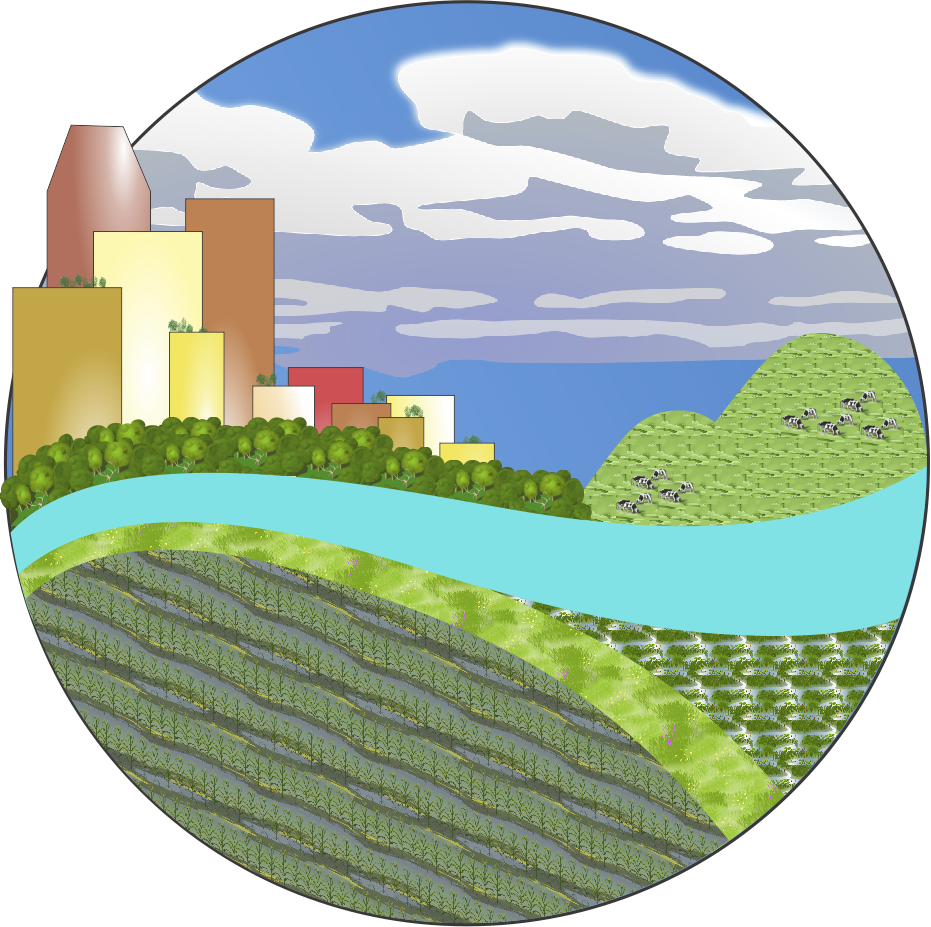
\includegraphics[height=3 in]{../imgs/updatedPewiLogo.png}
	\end{figure}
}
\author{PEWI team}
\date {\today} % date
\maketitle
\thispagestyle{empty} % no page number on cover
\end{titlepage}

% stuff before table of contents
\pagenumbering{roman}
\section*{Summary}
\addcontentsline{toc}{section}{\numberline{}Summary}
This is the document of index. This document includes all advanced tab description.
\cleardoublepage

\section*{Acknowledgements}
\addcontentsline{toc}{section}{\numberline{}Acknowledgements}
Thanks to so many people.
\cleardoublepage


%%%%%Table of content starts here
\tableofcontents
\thispagestyle{empty} % no page number on table of contents page
\cleardoublepage % no other contents on table of contents page

%%% to start page numbers from 1
\pagenumbering{arabic}
\setcounter{page}{1}

% === main contents ===

% Land Use section
\section{Land Use}\label{sec:landuse}
Upland grid cells, those not containing part of the river, are 10 acres (4 hectares) in area. Grid cells along the river decrease in area to account for the percent of the grid cell underwater. Land use for a particular land cover is calculated by the sum of the area of each grid cell using that land cover. To find percent land use, this sum is divided by the total area of the watershed and multiplied by 100.

% sub section
\subsection{Conventional Corn}

Corn performs best on gentle terrain with high drainage and low flooding probability. The conventional corn land cover in PEWI assumes conventional tillage and no use of cover crops, terraces, contours, grassed waterways, or stream buffers.

Strategic placement can maximize your per-unit yield: Muscatine 119, Tama 120B, Nicollet 55, and Clarion 138B soils are highly productive for annual crops in general, while Buckney 1636 and Gara-Armstrong 993E2 soils are unproductive.
 
With a conventional corn-dominated land cover, yield, erosion control, and nitrate, phosphorus, and sediment retention vary significantly under different precipitation scenarios. 

To improve ecosystem scores in extreme precipitation conditions, try switching from conventional to conservation crops.

Conventional crops also do not provide points in the wildlife habitat or carbon sequestration categories. To improve habitat scores, try adding some perennial or native habitat. To improve carbon sequestration scores, try adding some woody land covers or wetlands.


\subsection{Conventional Soy}

Soybeans perform best on gentle terrain with high drainage and low flooding probability. The conventional soybean land cover in PEWI assumes conventional tillage and no use of cover crops, terraces, contours, grassed waterways, or stream buffers. 
Strategic placement can maximize your per-unit yield: Muscatine 119, Tama 120B, Nicollet 55, and Clarion 138B soils are highly productive for annual crops in general, while Buckney 1636 and Gara-Armstrong 993E2 soils are unproductive.
 
With a conventional soy-dominated land cover, yield, erosion control, and nitrate, phosphorus, and sediment retention vary significantly under different precipitation scenarios. 

To improve ecosystem scores in extreme precipitation conditions, try switching from conventional to conservation crops.

Conventional crops also do not provide points in the wildlife habitat or carbon sequestration categories. To improve habitat scores, try adding some perennial or native habitat. To improve carbon sequestration scores, try adding some woody land covers or wetlands.

\subsection{Conservation Corn}

Corn performs best on gentle terrain with high drainage and low flooding probability. 

Strategic placement can maximize your per-unit yield: Muscatine 119, Tama 120B, Nicollet 55, and Clarion 138B soils are highly productive for annual crops in general, while Buckney 1636 and Gara-Armstrong 993E2 soils are unproductive.

Conservation corn base yield is equivalent to that of conventional corn.

One hundred percent conservation corn cover gives sediment retention scores above 90, and phosphorus retention and erosion control scores above 85 in all precipitation scenarios. Nitrate retention varies substantially under different precipitation scenarios. To improve nitrate retention scores in extreme precipitation conditions, try switching to perennial land uses.

Conservation crops provide minimal carbon sequestration and moderate habitat points. To improve carbon sequestration scores, try adding some woody land covers or wetlands. To improve habitat scores, try adding some native vegetation.

\subsection{Conservation Soy}

Soybeans perform best on gentle terrain with high drainage and low flooding probability. 

Strategic placement can maximize your per-unit yield: Muscatine 119, Tama 120B, Nicollet 55, and Clarion 138B soils are highly productive for annual crops in general, while Buckney 1636 and Gara-Armstrong 993E2 soils are unproductive.

Conservation soybean base yield is equivalent to that of conventional soybean.

One hundred percent conservation soybean cover gives sediment retention scores above 90, and phosphorus retention and erosion control scores above 80 in all precipitation scenarios. Nitrate retention varies substantially under different precipitation scenarios. To improve nitrate retention scores in extreme precipitation conditions, try switching to perennial crops.

Conservation crops provide minimal points in carbon sequestration, and moderate habitat points. To improve carbon sequestration scores, try adding some woody land covers or wetlands. To improve habitat scores, try adding some native vegetation.

\subsection{Alfalfa}

Alfalfa performs best on soils with excessive to moderate drainage.

Strategic placement can maximize your per-unit yield: Tama 120B, Muscatine 119, Tama 120C2, Nicollet 55, Nodaway 220, and Clarion 138B soils are highly productive for alfalfa and grass hay, while Buckney 1636, Okoboji 90, and Gara-Armstrong 993E2 soils are approximately half as productive.

Yield varies only slightly in extreme precipitation scenarios. 

One hundred percent alfalfa land cover gives the maximum score in nitrate retention, erosion control and sediment retention scores above 90, and phosphorus retention above 80 in all precipitation scenarios. Phosphorus contribution is decreased for areas with an elevation grade of less than 9%.

Alfalfa does not provide points in the habitat categories and provides only minimal carbon sequestration benefit. To improve habitat scores, try switching to grass hay or adding some native vegetation or stream buffers. To improve carbon sequestration scores, try adding some woody land covers or wetlands.

\subsection{Mixed Fruit and Vegetables}

Mixed fruit and vegetables perform best on fine sandy loam, silt loam, or loam. 

Strategic placement can maximize your per-unit yield: Buckney 1636, Downs 162D2, Nodaway 220, Ackmore-Colo 5B, Muscatine 119, and Gara-Armstrong 993E2 soils are highly productive for mixed fruit and vegetables, while all other soils are less than half as productive.

With a mixed fruit and vegetable land cover, erosion control, and nitrate, phosphorus, and sediment retention vary significantly under different precipitation scenarios. Yield is decreased in wet years. To improve these scores in extreme precipitation conditions, try switching to perennial or conservation crops.

As a collection of row crops, the mixed fruit and vegetable land cover attains nitrate retention scores similar to those of conventional and conservation corn and soybean. Similarly, it contributes little to carbon sequestration and therefore provides no points in that category. To improve carbon sequestration scores, try adding some woody land covers or wetlands.

As a high-input, high diversity land cover, mixed fruit and vegetables provide moderate points in biodiversity and high points in game wildlife.

\subsection{Grass Hay}

Grass hay performs best on soils with excessive to moderate drainage.

Strategic placement can maximize your per-unit yield: Tama 120B, Muscatine 119, Tama 120C2, Nicollet 55, Nodaway 220, and Clarion 138B soils are highly productive for alfalfa and grass hay, while Buckney 1636, Okoboji 90, and Gara-Armstrong 993E2 soils are approximately half as productive.

Yield varies only slightly in extreme precipitation scenarios.

One hundred percent grass hay land cover gives the maximum score in nitrate retention, while erosion control, and sediment and phosphorus retention score above 95 in all precipitation scenarios.

As a stream buffer and low input land use, grass hay provides moderate points in the habitat categories. To improve habitat scores, try adding some native vegetation. Grass hay provides minimal carbon sequestration benefit.  To improve carbon sequestration scores, try adding some woody land covers or wetlands.

\subsection{Switchgrass}

Switchgrass is highly adaptable to soil type. Muscatine 119, Tama 120B, Nicollet 55, Nodaway 220, Clarion 138B, Canisteo 507, and Coland 135 soils are all highly productive for switchgrass. Switchgrass is also productive on soil types that have minimal yield in corn or soy land covers, including Buckney 1636, Okoboji 90, Downs 162D2, and Gara-Armstrong 993E2 soils.

Yield varies only slightly in extreme precipitation scenarios.

One hundred percent grass hay land cover gives the maximum score in sediment retention, erosion control, and nitrate retention, with phosphorus retention scores above 95 in all precipitation scenarios.

As a stream buffer, grassland and low input land use, switchgrass provides points in the habitat categories. To improve habitat scores, try adding some native vegetation including wetland and conservation forest. Switchgrass provides moderate carbon sequestration benefit.  To improve carbon sequestration scores, try adding some woody land covers or wetlands.

\subsection{Permanent Pasture}

Permanent pasture performs best on soils with excessive to moderate drainage.

Strategic placement can maximize your per-unit yield: Tama 120B, Muscatine 119, Tama 120C2, Nicollet 55, Nodaway 220, and Clarion 138B soils are highly productive for alfalfa and grass hay, while Buckney 1636, Okoboji 90, and Gara-Armstrong 993E2 soils are approximately half as productive.

Yield varies only slightly in extreme precipitation scenarios, but is much higher for rotational grazing land cover than for permanent pasture land cover. To improve yield, try switching from permanent pasture to rotational grazing.

One hundred percent permanent pasture cover gives the maximum score in nitrate retention, with erosion control scores and sediment retention scores above 90, and phosphorus retention scores above 80 in all precipitation scenarios. 

Permanent pasture does not provide points in the habitat categories. To improve habitat scores, try switching to the rotational grazing land cover. Permanent pasture provides minimal carbon sequestration benefit.  To improve carbon sequestration scores, try adding some woody land covers or wetlands.

\subsection{Rotational Grazing}

Rotational grazing performs best on soils with excessive to moderate drainage.

Strategic placement can maximize your per-unit yield: Tama 120B, Muscatine 119, Tama 120C2, Nicollet 55, Nodaway 220, and Clarion 138B soils are highly productive for rotational grazing and permanent pasture, while Buckney 1636, Okoboji 90, and Gara-Armstrong 993E2 soils are approximately half as productive.

Yield varies only slightly in extreme precipitation scenarios, but is much higher for rotational grazing land cover than for permanent pasture land cover.

One hundred percent rotational grazing cover gives the maximum score in nitrate retention, with erosion control scores above 95, sediment retention scores above 90, and phosphorus retention scores above 85 in all precipitation scenarios.

As a stream buffer, grassland, and low input, high diversity land use, rotational grazing provides the highest level of points in the game wildlife category and relatively high points in the biodiversity category. To improve habitat scores, try diversifying the watershed cover by adding some native vegetation. Rotational grazing provides minimal carbon sequestration benefit.  To improve carbon sequestration scores, try adding some woody land covers or wetlands.

\subsection{Wetland}

Wetlands have a high rate of carbon sequestration in PEWI that applies to all land in the wetland cover type. The biodiversity benefits and nitrate reduction associated with wetland use are optimized by using Strategic Wetlands, located in flat, poorly drained areas of the watershed. Strategic Wetlands may be prairie potholes, or low spots in the left lobe of the watershed, or shallow areas along the river. As a native, high diversity, low input land cover, it provides the highest level of habitat benefits. Game Wildlife benefits from wetlands are derived from percent area of land coverage, as well as using wetland or another stream buffer in appropriate cells. 

\subsection{Prairie}
One hundred percent prairie land cover gives the maximum score in sediment retention, erosion control, phosphorus retention, and nitrate retention.

Prairie has a moderate rate of carbon sequestration in PEWI that applies to all land in the prairie cover type. To improve carbon sequestration scores, try incorporating woody land covers or wetlands.

As a native, high diversity, low input land cover, it provides the highest level of habitat benefits. Game Wildlife benefits from prairie are derived from percent area of land coverage, as well as using prairie or another stream buffer in appropriate cells. Use a diverse mix of prairie and other native vegetation to maximize habitat scores.


\subsection{Conventional Forest}
Forest land covers perform best on well drained, moderately deep, or moderately wet soils, and are least productive in wet, sandy, saline, or sodic soils.

Strategic placement can maximize your per-unit yield: Gara-Armstrong 993E2 and Downs 162D2 soils are highly productive for forest land covers but perform poorly for annual crops. The conventional forest land cover maximizes wood yield.

As a perennial crop, the conventional forest land cover attains maximum nitrate retention scores. It achieves erosion control, sediment retention, and phosphorus retention scores above 97% in all precipitation scenarios. 

Conventional forest land cover provides high points in the carbon sequestration category. To improve carbon sequestration further, include some short-rotation woody land cover.

\subsection{Conservation Forest}
Forest land covers perform best on well drained, moderately deep, or moderately wet soils, and are least productive in wet, sandy, saline, or sodic soils.

Strategic placement can maximize your per-unit yield: Gara-Armstrong 993E2 and Downs 162D2 soils are highly productive for forest land covers but perform poorly for annual crops. The conventional forest land cover maximizes wood yield.

As a perennial crop, the conservation forest land cover attains maximum nitrate scores. It achieves erosion, sediment, and phosphorus control scores above 97\% in all precipitation scenarios. 

Conservation forest land cover provides high points in the carbon sequestration category. To improve carbon sequestration further, include some short-rotation woody land cover.

As a native, high diversity, low input land cover, the conservation forest land use provides the highest level of habitat benefits. To maximize habitat scores, try diversifying the watershed by including some other native vegetation covers.


\subsection{Short-Rotation Woody Bioenergy}
In PEWI, short rotation woody crops perform equally well in all soil, topography, and precipitation scenarios. One hundred percent short-rotation land cover gives the maximum score in carbon sequestration, water and soil quality scores of over 95, and moderate habitat scores.

% Physical Features section
\newpage
\section{Physical Features}\label{sec:physicalfeatures}
In the Physical Features tab, you'll find information on topography, soil properties, subwatershed boundaries, and strategic wetland areas. These properties can help you strategize the placement of land uses. Physical features influence the Ecosystem Services gained from each land cover choice, from soil and water quality improvement to yield.

% sub section
\subsection{Topographic Relief}

Topography influences water runoff patterns, which in turn influences gross erosion, sediment retention, and phosphorus retention scores.

Slope length steepness is also contingent on topography and can range from a factor of .05 to 2.20. See the Erosion Control tab for information about Slope length steepness factor and its role in erosion calculations. Topography also affects the support practice factor in erosion calculations for conservation corn and soy, since terracing and contouring are assumed for elevation grades above 2\%. \cite{24}

The runoff factor for phosphorus incorporates Runoff Curve Numbers, which in turn depend on topographic relief. For more information on these calculations, please see the Sediment and Phosphorus tabs.

\subsection{Flood Frequency}
This feature shows the frequency of flooding for each PEWI grid cell, as found in the Iowa Soil Properties and Interpretations Database (ISPAID) Soil Survey.\cite{25}  Flooding categories are defined below, according to the ISPAID manual. In PEWI, flooding frequency is incorporated into yield calculations: yield is determined as per ISPAID calculations as a function of CSR2 results. The CSR2 formula is CSR2 = S-M-W-F-D+/- EJ, where F is the field condition including ponding and flooding properties, among other factors.\cite{26}  See the Yield tab for more information.
\begin{itemize}
\item NONE	=	0	=	Flooding is not probable.
\item RARE	=	10	=	Flooding is unlikely but possible under unusual weather conditions.
\item OCCAS	=	20	=	Flooding occurs on an average of 50 times or less in 100 years.
\item FREQ	=	40	=	Flooding occurs on an average of more than 50 times in 100 years.
\item PONDED	=	50	=	Standing water on soils in closed depressions.  Unless the soils are artificially drained, the water can be removed only by percolation or evapotranspiration.  (Ponded is for short duration unless otherwise specified).
\end{itemize}

\subsection{Strategic Wetlands}
There are 20 strategic wetlands in PEWI. These include “prairie potholes” in the lower lobe of the watershed that are prone to flooding, but have poor drainage, and shallow areas along the river or a tributary that would regularly have high moisture content in the soil. Utilizing strategic wetlands by planting Wetland in these areas leads to a significant improvement in ecological services.

Wetlands including prairie pothole wetlands and stream buffer wetlands provide native habitat for amphibians, invertebrates, and birds including ring-necked pheasants and mallards,\cite{27}  increasing biodiversity and game wildlife services. It also curbs nitrate pollution; for subwatersheds with at least one strategic wetland, nitrate loss is cut by 52\%.\cite{28}


\subsection{Subwatershed Boundaries}
This feature depicts the boundaries of each subwatershed, which are important in water runoff patterns influencing nitrate loss. Subwatershed boundaries were realistically calculated based on topographic modeling for the watershed. 

\subsection{Drainage Class}

This feature shows the relative drainage of each pixel in PEWI. Drainage classes are defined below, according to the Iowa Soil Properties and Interpretations Database (ISPAID) manual.\cite{29}  In PEWI, drainage class influences phosphorus, and ISPAID yield values incorporate drainage class information; for more information see the Yield tab.\cite{30} The subsurface drainage component (SDC) of the phosphorus delivery calculation is a function of flow factor (FF), which is dependent on drainage class. Additionally, the runoff component of the phosphorus calculation incorporates runoff curve numbers based on hydrologic group. See the Phosphorus Tab and Hydrologic Group Tab for more information. 

\begin{itemize}
\item E	=	10	=	Excessive
\item E-SE	=	15	=	Excessive-Somewhat excessive
\item SE	=	20	=	Somewhat excessive
\item SE-W	=	25	=	Somewhat excessive-Well
\item W	=	30	=	Well
\item W-MW	=	35	=	Well-Moderately well
\item MW	=	40	=	Moderately well
\item MW-SP	=	45	=	Moderately well-Somewhat poor 
\item SP	=	50	=	Somewhat poor
\item SP-P	=	55	=	Somewhat poor-Poor
\item P	=	60	=	Poor
\item P-VP	=	65	=	Poor-Very poor
\item VP	=	70	=	Very poor
\end{itemize}
\subsection{Soil Class}
There are thirteen soil classes in PEWI. Each soil class has its own set of properties, including percent slope, flood frequency, drainage class, hydrologic group, soil texture, Corn Suitability Rating, and taxonomic classification. The class of a soil can tell you about its physical and chemical composition, which influences its behavior and production capacity in various situations. 
\subsubsection{Hydrologic Group}
The following chart includes each hydrologic group as defined by the ISPAID Manual.
\begin{itemize}
\item Group A	=	Soils having a high infiltration rate (low runoff potential) when thoroughly wet.  These consist mainly of deep, well drained to excessively drained sands or gravely sands.  These soils have a high rate of water transmission.
\item Group B	=	Soils having a moderate infiltration rate when thoroughly wet.  These consist chiefly of moderately deep or deep, moderately well drained or well drained soils that have moderately fine texture to moderately coarse texture.  These soils have a moderate rate of water transmission.
\item Group C	=	Soils having a slow infiltration rate when thoroughly wet.  These consist chiefly of soils having a layer that impedes the downward movement of water or soils of moderately fine texture or fine texture.  These soils have a slow rate of water transmission.
\item Group D	=	Soils having a very slow infiltration rate (high runoff potential) when thoroughly wet.  These consist chiefly of clays that have a high shrink-swell potential, soils with a permanent high water table, soils that have a clay pan or clay layer at or near the surface, and soils that are shallow over nearly impervious material.  These soils have a very slow rate of water transmission.
\end{itemize}

\subsection{Soil Texture}
Texture refers to the composition of the soil, including organic matter content and particle size distribution. Abbreviations for texture types used in the ISPAID are below.
\begin{itemize}
\item C                =    Clay
\item CL              =    Clay loam
\item CN-SIL       =    Channery silt loam
\item CO-SICL     =    Cobbly silty clay loam
\item CS              =    Coarse sand
\item CSL            =    Coarse sandy loam
\item FS              =    Fine sand
\item FSL            =    Fine sandy loam
\item GR-SL        =    Gravelly sandy loam
\item L                =    Loam
\item LS              =    Loamy sand
\item LFS            =    Loamy fine sand
\item MK             =    Muck
\item MK-SICL    =    Mucky silty clay loam
\item MK-SIL       =    Mucky silt loam
\item S                =    Sand
\item SIC             =    Silty clay
\item SICL           =    Silty clay loam
\item SIL             =    Silt loam
\item SL              =    Sandy loam
\item SP              =    Sapric
\item VFSL          =    Very fine sandy loam
\end{itemize}
A table of soil texture by soil type is below.

\begin{center}
\begin{tabular}{ |c|c|c|c| } 
\hline
County & ISPAID Soil Type & Texture \\
\hline
\multirow{3}{7em}{Boone County} & Clarion 138B & L \\ 
& Buckney 1636 & FSL \\ 
& Canisteo 507 & SICL \\ 
& Coland 135   & CL  \\
& Nicollet 55  & L   \\
& Okoboji 90   & MK-SIL \\
\hline
Jasper County & Downs 162D2 & SIL \\
& Gara-Armstrong 993E2 & L \\
& Ackmore-Colo 5B & SIL\\
& Tama 120C2 & SICL \\
& Tama 120B  & SICL \\
& Muscatine 119 & SICL \\
& Nodaway 220 & SIL \\
\hline
\end{tabular}
\end{center}
\subsection{Corn Suitability Rating}
The CSR2 calculates the corn suitability value as:
CSR2 = S-M-W-F-D +/- EJ
\begin{itemize}
\item Where S is the taxonomic subgroup class of the soil 
\item M is the family particle size class (soil particle composition)
\item W is a function of the soil’s water holding capacity
\item F is the field condition factor, including slope, erosion class, flooding, and topsoil thickness
\item D incorporates soil depth and “T factor,” or soil loss tolerance
\item EJ is an expert judgment factor accounting for series abnormalities such as textural extremes or high bulk density.\cite{32} 
\end{itemize}

% Precipitation section
\newpage
\section{Precipitation}
Precipitation is based on historical annual precipitation data from Iowa to simulate climate variability. Scenarios are broken into three categories. 
\begin{itemize}
  \item The Dry category includes the 62.4 cm/yr (24.58 in/yr) scenario, with a probability of 5\%, and the 71.6 cm/yr (28.18 in/yr) scenario, with a probability of 15\%. 
  \item The Normal category includes the 77.2 cm/yr (30.39 in/yr) scenario, with a probability of 15\%, the 81.7 cm/yr (32.16 in/yr) scenario, with a probability of 15\%, and the 87.2 cm/yr (34.34 in/yr) scenario, with a probability of 15\%.
  \item The Wet category includes the 92.6 cm/yr (36.47 in/yr) scenario, with a probability of 15\%, and the 114.6 cm/yr (45.1 in/yr) scenario, with a probability of 5\%.
\end{itemize}

In PEWI, the level of precipitation influences water quality and soil quality metrics including nitrate and phosphorus runoff, gross erosion, and sediment transport. This is because improved water flow carries a greater quantity of soil and nutrients downstream. Extremes in precipitation also decrease yield for annual crops, mixed fruits and vegetables, alfalfa, grass hay, switchgrass, permanent pasture, and rotational grazing.\cite{33}  Calculations for yield for each land use can be found in the corresponding yield tab.


% Management Practices section
\newpage
\section{Management Practices}
Here you’ll find information on management practices used in PEWI’s calculations.
\subsection{Crop Rotation}
A complete chart for Cover Management Factor is found below:
\begin{center}
\begin{tabular}{ |c|c|c|c|c| } 
\hline
\multirow{5}{3em}{Cover Management Factor} & Cij & Conventional Corn preceding annual row crop: & 0.085 - 0.200 \\ 
& & 0.085, \textit{Conservation Corn} & \\ 
& & 0.116, \textit{Conservation Soybean} & \\ 
& & 0.150, \textit{Conventional Corn} & \\
& & 0.200, \textit{Conventional Soybean}  & \\
& & 0.200, \textit{Mixed Fruit and Vegetables} & \\
& & Conservation Corn preceding annual row crop:  & 0.020-0.116\\
& & 0.020, \textit{Conservation Corn}  & \\
& & 0.031, \textit{Conservation Soybean} & \\
& & 0.085, \textit{Conventional Corn} & \\
& & 0.116, \textit{Conventional Soybean} & \\
& & 0.116, \textit{Mixed Fruit and Vegetables} & \\
& & Conventional Soybean/Mixed Fruit and Vegetables 
preceding annual row crop: & 0.156-0.300\\
& & 0.156, \textit{Conservation Corn} & \\
& & 0.178, \textit{Conservation Soybean} & \\
& & 0.260, \textit{Conventional Corn} & \\
& & 0.300, \textit{Conventional Soybean} & \\
& & 0.300, \textit{Mixed Fruit and Vegetables} & \\
& & Conservation Soybean preceding annual row crop: & 0.052-0.178\\
& & 0.052, \textit{Conservation Corn} & \\
& & 0.055, \textit{Conservation Soybean} & \\
& & 0.156, \textit{Conventional Corn} & \\
& & 0.178, \textit{Conventional Soybean} & \\
& & 0.178, \textit{Mixed Fruit and Vegetables} & \\

\hline
\end{tabular}
\end{center}

% Modules section
\newpage
\section{Modules}
The scientific modules in PEWI display ecosystem service scores, the benefits that the watershed provides to people. PEWI tracks ecosystem services in four categories: 
\begin{itemize}
\item Habitat
\item Soil Quality
\item Water Quality
\item Yield
\end{itemize}
\subsection{Habitat}
This category includes two Habitat metrics. Providing habitat to a multitude of species is important for water quality, nutrient recycling, pollination, and biocontrol, including suppression of pests that decrease crop production. A highly diverse ecosystem is also more highly adaptable to regional and global stressors and extreme disturbances, such as fires or flooding.

\subsubsection{Biodiversity}
Biodiversity is expressed on a 0-10 scale and calculated from a composite score of three nested categories and two location-specific categories. 
\begin{itemize}
\item 1.5 points maximum awarded for percentage of watershed area in low-input and/or high diversity land uses, conservation annual crops, or permanent pasture. 
\item 1.5 points maximum awarded for percentage of watershed area in high-diversity land uses. 
\item 4 points maximum awarded for percentage of watershed area in native land uses. 
\item 1.5 points maximum awarded for wetland coverage and strategic use. 
\item 1.5 points maximum awarded for using a stream buffer with an appropriate land use type (conservation crop, forest, grass hay, switchgrass, mixed fruit and vegetable, prairie, rotational grazing, short-rotation woody bioenergy, or wetland). Biodiversity is maximized when each of these criteria is fulfilled and minimized in conventional annual crop scenarios.
\end{itemize}


\subsubsection{Game Wildlife}
Game wildlife is expressed on a 0-10 scale and calculated from six categories. 
\begin{itemize}
\item 1.5 points maximum awarded for percentage of watershed area in low-input and/or high diversity land uses, conservation annual crops, or permanent pasture. 
\item 4 points maximum awarded for percentage of watershed area in high diversity land uses. 
\item 1.0 points maximum awarded for at least 5% area in conservation forest.
\item 1.0 points maximum awarded for at least 5% area in grasslands.
\item 1.0 points maximum awarded for at least 5% area in wetlands.
\item 1.5 points maximum awarded for percentage of stream buffers with appropriate land use types (conservation corn, conservation soybean, forest, grass hay, switchgrass, mixed fruit and vegetable, prairie, rotational grazing, short-rotation woody bioenergy, or wetland).
\end{itemize}
  
\subsection{Soil Quality}
 Soil quality is important for agricultural production and ecosystem health. PEWI monitors two metrics of soil quality: carbon sequestration and erosion prevention. Soils have an immense carbon-holding capacity and, through the actions of plants and microbes, can reduce air pollutant levels. Protecting soils can also minimize erosion, which can diminish crop productivity and deteriorate aquatic stream habitat.\cite{36} 
 
 \newpage
\subsubsection{Carbon Sequestration}
The annual carbon sequestration of the watershed is calculated as the sum, as land-use type i goes from 1 to n, of the product of land-use type area and the associated rate of sequestration, based on Fissore et al. and Al-Kaisi, Yin, and Licht.\cite{37} 
A complete chart for Cover Management Factor is found below:
\begin{center}
\begin{tabular}{ |c|c|c|c|c| } 
\hline
Source & Annual Row\\
& Crop Types & Measured Unit & PEWI Land-use Types
& Values \\
& & & & (Mg ha-1 yr-1) \\
\hline
\multirow{3}{3em}{Fissore et al. (2010)} & Forests & Total biomass and soils & Conservation Forest, \\
& & & Conventional Forest & 3.67 \\ 

& Incorporation of cover crops 
& Soils & Conservation Corn, \\
& & & Conservation Soybean & 0.40\\ 
\hline

& Perennial Grassland 
& Soils & Prairie & 1.07\\ 
\hline

& Pasture or hay land 
& Soils & Grass hay, Permanent \\
& & &  pasture, Rotational grazing & 0.29\\
\hline

& Prairie Potholes
& Soils & Wetland & 3.05\\
\hline

& Short-Rotation \\
& Woody Crops & Total Biomass \\
& & and Soils & Short-Rotation & 4.69 \\
\hline
 
Al-Kaisi \\
et al.\\
(2005) & Switchgrass & soil depth \\ [-0.43 in]
& & SOC, 0-15 cm & Herbaceous\\
& & & Perennial Bioenergy & 1.20 \\
\hline

& Corn-Soy \\
& Alfalfa Rotation & SOC, 0-15 cm \\
& & soil depth & Alfalfa & 0.50 \\
\hline
\end{tabular}
\end{center}
 
 
\cleardoublepage
\newpage

\subsubsection{Erosion Control}
The Erosion Control module is based on guidelines from the 2004 Iowa Phosphorus Index. Gross Erosion is the soil loss per year from ephemeral gully erosion, rill erosion, and interrill erosion; a high gross erosion corresponds to a low soil retention, and low gross erosion to a high soil retention. Excessive soil erosion has been shown to decrease soil and water quality, leading to diminished crop productivity and deterioration of aquatic stream habitat.\cite{36}

\subsection{Water Quality}
Water quality is a salient issue for Corn Belt states and other agricultural regions. PEWI tracks three metrics of water quality: nitrate, sediment, and phosphorus. Nitrate-N concentrations in drinking water exceeding the Environmental Protection Agency’s National Regulation limit of 10 mg/L can lead to negative health effects, including blue baby syndrome.\cite{37}  Downstream, nitrate-N loading also creates hypoxic (low-oxygen) zones in gulf regions, leading to loss of marine life.\cite{38}  Sediment delivery impacts water quality both locally and downstream.\cite{39} Phosphorus loss impacts local producers who incur expenses of phosphorus fertilizer application, regional aquatic ecosystems and human economy through freshwater eutrophication, and distant scales through gulf hypoxia.\cite{40} 

\subsubsection{Nitrate Retention}
Nitrate pollution is a well-known public health problem that negatively affects human health when exceeding a contamination level of 10 mg L-1 in drinking water, which is the limit established in the National Primary Drinking Water Regulations.  It also harms aquatic ecosystems by depleting oxygen in the Gulf of Mexico.\cite{41}

\subsubsection{Phosphorus Retention}
Phosphorus transport from fields to surface water can threaten aquatic species and human economy due to aquatic eutrophication. In PEWI, Phosphorus Retention is the indexed inverse of annual in-stream phosphorus loading, with high phosphorus runoff corresponding to low phosphorus retention, and vice versa.

\subsubsection{Sediment Control}
Sediment transport can adversely affect water quality both at the local level and downstream. Sediment control is the indexed inverse of annual in-stream sediment delivery. 

\subsection{Yield}
Yields are based on modifications to Corn Suitability Rating, determined by the CSR2 from Iowa State University. The CSR2 assigns a corn suitability rating to each soil type in Iowa, and this data is incorporated into PEWI grid cells. Yields from other crops are estimated as a proportion of corn yield values. 

\subsubsection{Corn Yield}
The Corn Grain yield in PEWI assumes high-level management, and no difference between yield in conventional and conservation systems. Corn grain yield is based on the Iowa Soil Properties and Interpretations Database (ISPAID) equation of Corn Yield = (1.6 * Corn Suitability Rating) + 80, and multiplied by a conversion factor of 0.0254 Mg/bu.\cite{42}  
 Total production is given by the product of the yield on a per-unit basis and the area of the grid cell, summed over the entire watershed. 
 
\subsubsection{Soybean Yield}
Soybean yield is based on the Iowa Soil Properties and Interpretations Database (ISPAID) equation of Soybean Yield = 0.29 * Corn Yield. Total production is given by the product of the yield on a per-unit basis and the area of the grid cell, summed over the entire watershed. 

\subsubsection{Alfalfa Hay Yield}
Alfalfa Hay yield is based on the Iowa Soil Properties and Interpretations Database  (ISPAID) equation of YBij[Alfalfa] = DFij * Corn Yield multiplied by a conversion factor from tons to megagrams and with a minimum of 8.07 Mg/ha yr.\cite{43} 

DFij is a drainage factor equal to:
\begin{itemize}

\item 0.028 for soils with Drainage Class values of 10-35, as well as most soils with Drainage Class values of 40
\item 0.026 for soils with Drainage Class values of 45-50, as well as two soils with Drainage Class values of 40
\item 0.021 for soils with Drainage Class values of 55-70

\end{itemize}

Total production is given by the product of the yield on a per-unit basis and the area of the grid cell, summed over the entire watershed. 

\subsubsection{Grass Hay}
Grass Hay yield is based on the Iowa Soil Properties and Interpretations Database (ISPAID) equation of YBij[GrassHay] = DFij * CornYield multiplied by a conversion factor from tons to megagrams and with a minimum of 8.07 Mg/ha yr.\cite{43} 

DFij is a drainage factor equal to:

\begin{itemize}

\item 0.028 for soils with Drainage Class values of 10-35, as well as most soils with Drainage Class values of 40
\item 0.026 for soils with Drainage Class values of 45-50, as well as two soils with Drainage Class values of 40
\item 0.021 for soils with Drainage Class values of 55-70

\end{itemize}

Total production is given by the product of the yield on a per-unit basis and the area of the grid cell, summed over the entire watershed. 

\subsubsection{Cattle Yield}
Cattle yield is based on the Iowa Soil Properties and Interpretations Database (ISPAID) equation of Alfalfa-Grass Hay Yield, with a conversion from Alfalfa-Grass yield to head of cattle.

\subsubsection{Mixed Fruit and Vegetable Yield}
Yield for mixed fruit and vegetables is determined from an estimate for grapes, strawberries, green beans, and squash, with each grid cell divided evenly among the four crops. 

\subsubsection{Wood Yield}
Wood production is based on estimates generated using the 2007 Iowa Woodland Suitability Composite.\cite{44} Yield estimates assume appropriate selection of tree species for a given location. A 30\% reduction in wood production estimates for conservation forest is applied to account for differences in management.

\subsubsection{Switch Grass Yield}
Switchgrass biomass yields are based on a modification to Iowa Soil Properties and Interpretations Database (ISPAID) corn suitability ratings.\cite{45}

\subsubsection{Woody Biomass}
Woody biomass yield estimates are based on a 10-year aspen biomass of 224 Mg/ha.\cite{46}  Annual production assumes temporally spaced plantings such that a constant 22.4 Mg/ha is harvested each year.

\newpage

\section{Functionality}
This section describes how to navigate the PEWI application, including play mode options and watershed editing tools.

\subsection{Navigating the PEWI Workspace}
Opening Sandbox or playing a PEWI Level brings you to the PEWI Workspace. In the workspace, there are many tools that you can use to edit the watershed and monitor ecosystem services.

\subsubsection{Tool Panel}
The tool panel has seven features to use in designing your watershed. The Land Use tab includes 15 land cover options to use in your watershed, ranging from annual and perennial crops to pasture, forests, and native land cover.

The Precipitation tab shows the precipitation for each year. PEWI simulates real life by choosing randomly from seven precipitation levels. To override the presets, select a precipitation level from the drop-down menu.

The Years tab allows you to add another year of simulation to your watershed. Some of the impacts of land use choices vary with weather or previous practices. You can explore these effects by playing across multiple years.

The Indicator Tab includes overlay maps for Nitrate, Erosion, and Phosphorus risk. You can edit the land use while in overlay mode to target a specific risk area.

The Physical Features tab includes five watershed behavior overlay maps displaying flood frequency, strategic wetland areas, subwatershed boundaries, drainage class, and soil class. You can edit the land use while in overlay mode to target a specific region.

The Yield Tab allows you to strategically place landuse types on the map, by providing information for each yield type and their respective yield base rates based off soil type. To learn more about this feature, check out the Yield Tab video.

The buttons located above the Toolbar are for placing landuse types on the map. The leftmost button is the individual brush, allowing you to paint one landuse type at a time. The middle button allows you to paint multiple tiles at once by dragging and clicking the corners. The arrow button is the Undo button, allowing you to undo previous changes. Any amount of previous changes can be undone. You can also undo changes by pressing the "U" hotkey on the keyboard. 

\subsubsection{Results Panel}
The results page provides data visualization and numerical results for your watershed design.

\paragraph{Land Use Graph}
The first circle graph gives the percent of the watershed you’ve devoted to each of the land uses. Scroll over the graph or the legend on the right to view the quantitative data for that land use. Use the up and down arrows to switch between List view and Category view. List view displays each land use individually. Category view groups land uses into seven categories: annual grain, annual legume, mixed fruit and vegetables, pasture, non-pasture perennial herbs, perennial legume, and perennial wetland. Use the arrows to switch between years. 

\paragraph{Ecosystem Services Graph}
The ecosystem services radar plot shows the zero-to-100 score of ecosystem services pertaining to water quality, soil health, and habitat. A watershed design with high scores in many ecosystem services will produce a radar plot shape with a large area, while a watershed design with low ecosystem service scores will produce a smaller shape. 

\paragraph{Precipitation Graph}
The precipitation graph shows the amount of precipitation for each year of the simulation. 

\paragraph{Data Sheet}
Click on the abacus icon at the top of the Results page to access the data tab with two numerical tables. Both tables provide three metrics: the zero-to-100 scale used in the Scores tab, English units, and metric units. The first table gives the percent area of each land use by year, and the second gives ecosystem service scores by year. At the bottom of the page are precipitation data and strategic wetland use for each year. 

\subsubsection{Comment Panel}
Click the comment bubble to show or hide the comment panel. In Level mode, the comment panel will show instructions for completing the next objective in the level. 

\subsubsection{Index Information Box}
The Index Information Box is located at the bottom right portion of the screen. Each tab is given particular information about their intended usage and each individual feature for each tab is given some information in the Index Box and where to learn more, by directing the User to its respective Index entry. Every tab, from the Landuse Tab to the Yield Tab has information. Check them out! 

\subsubsection{View Perspective}
Press or hold D to rotate the watershed clockwise.
Press or hold A to rotate the watershed counterclockwise.
Press or hold W to pivot your viewpoint toward the horizon (flat)
Press or hold S to pivot your viewpoint toward the perpendicular
Right click to rotate the canvas with your mouse.

Use the up and down arrow keys to zoom in and out.
Use the left and right arrow keys to pan left and right.

Press T to toggle 3-D topographical view.

Press E to reset the camera position to default.

\subsubsection{Save Watershed}
Click the download icon in the upper right-hand corner to save your watershed to your computer. Upload to continue with your design.

\subsection{Main Menu}
Select Sandbox to explore the watershed on your own.
Select Play to play an interactive PEWI level.
Select Utilities to design a level, set up Multiplayer Mode, or aggregate Multiplayer Maps.
For more information, see the Levels tab and Multiplayer Mode tab.

\subsection{Guided Play}
PEWI comes with predesigned, thematic levels, ranging from introductory to complex. The N-Factor (Nitrogen) set focuses on the interaction between nitrate levels, physical features, land uses, and other ecosystem service scores. The P-Factor (Phosphorus) focuses on improving phosphorus, sediment, and erosion levels. The B-Factor (Biodiversity) focuses on habitat variety and suitability.

To create your own level, choose Design a Level from the Utilities menu. You can write a customized lesson with your own objectives and board presets.

\subsection{Multiplayer Mode}
PEWI offers a Multiplayer Mode. Under Utilities, click on the "Set-Up Multiplayer" button. In Multiplayer Mode, up to 6 Players can be added. Click on the Player numbers to draw out boundaries for each Player on the map with the brush tools.

You can also merge and combine Player boundaries and add and remove Players. Once finished, press "V" to download a Multi-Map file. Return to sandbox and click on the down arrow on the upper right part of the screen. Click on Upload and select a Player from your map files. In this case, Player 1 will be given only their boundaries drawn out for them to paint landuse types on. Scores in the Results are adjusted for these sections.

You can continue to adjust any Player maps as seen fit. Once finished, hit download to update the maps. To see all of the maps put together at once, go to "Utilities" and "Aggregate Multi-Maps". Add the files that have been changed and download the aggregate maps. Go back to "Sandbox" and upload the combined map file.

\subsection{Pause Menu}
The Pause Menu can be accessed by pressing the "Escape Key" Clicking on the Index will take you to the various Index Entries, where you can learn about different features of PEWI with videos The "Instructor Options" feature can also be accessed where customizations can be made and are further explored in the "Instructor Options" video The final part of the Pause Menu is the "Main Menu" feature, where you can go back to PEWI's main menu.

\subsection{Hover Information}
Specific information can be shown when hovered over tiles on the map. Each map when hovered over will display the tile's coordinates, the Land Cover that is currently being placed on the map, Precipitation level, and Soil Type. On some maps, there are some additional bits of information when hovered over. For the Nitrate, Erosion, and Phosphorus Maps, raw scores will show up that correspond to their map keys. Strategic Wetlands and Subwatershed Boundaries have their sections appear, while Flood Frequency, Drainage and Soil Class have their map key information appear. Yield maps all have their raw scores appear as well. Hover information displayed can be customized in the Instructor Options page and can be toggled on and off accordingly.  

\subsection{Hotkeys}
\begin{itemize}
\item Shift + Click	Fill the watershed with the selected land type
\item E	Reset camera position
\item Escape	Access Pause Menu
\item R	Randomize all land use types
\item T	Toggle topographical view
\item U	Undo previous land change
\item O	Toggle previous overlay
\item B	Toggle recording feature
\item V	Create multiplayer maps in multiplayer utility
\item D	Rotate clockwise
\item A	Rotate counterclockwise
\item W	Pivot toward the horizon (flat)
\item S	Pivot toward the perpendicular
\item Q	Toggle Flying Mode
\item Use the up and down arrow keys to zoom in and out
\item Use the left and right arrow keys to pan left and right
\item Right Click	Rotate watershed with your mouse
\end{itemize}

\subsection{Hotkey Customization}
By pressing the Esc Key and going to Instructor Options, a list of Hotkeys is available with their default settings. However, the hotkeys can be customized and adjusted as much as possible, with the option of having two hotkeys per feature. You can also reset the hotkeys to bring them back to their default settings. 

\subsection{Randomization}
Press "R" to randomize the landuse tiles on the watershed. The watershed can be randomized an infinite number of times. Press the Esc key to go to Instructor Options, where you can turn off landuse types. By turning off Conventional Corn, the landuse type will no longer appear when randomized. This applies for any other landuse types that are turned off. Landuse types can be turned back on and put back into randomization through the Instructor Options as well. 

\subsection{Undo Function}
In PEWI, there is an undo function that allows you to undo changes to the map, such as painting tiles or randomizing the map. Once you want to make changes to your previous edits to the map, click on the undo button, located next to the paint brush buttons above the tool box. You can also undo your changes by pressing the "Undo Hotkey" which is "U" on the keyboard. You can undo up to your oldest change to the map. The undo hotkey also extends to painting multiple tiles at once. 

\subsection{Print Function}
You can print your maps, results, and much more with Pewi. Activate the Print function by pressing "P" on the keyboard and select what you want to be printed out on a PDF. There are plenty of categories to choose from to print, including: Landuse Type Maps for set years, results, levels maps, and much more. Buttons such as "Select All" and "Reset" can help you choose. Once finished, you can click "Preview PDF" to see what will be on your PDF and then "Download" when ready. You can then print out your PDF once you save it. When you're finished, click "Exit". 

\subsection{Record}
By pressing B, you can record your actions with PEWI. The record feature will keep track of all actions. When you're done recording, press B again to save what was recorded. If you want to see your recording, go back to the main menu and click on "Utilities", then "Run User Simulation" where you can upload your recording. Once clicking "Click here to begin Simulation", you can view your recording. A bar at the bottom left of the screen will show the recording's progress and it's possible to fast forward and rewind. Once finished, you can replay or return to the Main Menu. 

\subsection{About}
People in Ecosystems/Watershed Integration (PEWI) is a simple web-based educational game designed to provide a scientific platform for teaching, discussing, and evaluating the tradeoffs associated with agricultural land use and management. Players iteratively manipulate land use annually for three years in a virtual 6000 acre watershed to meet a variety of goals. The tool computes a variety of results, including agricultural yields, soil erosion, stream pollution, and wildlife habitat.

PEWI v3 is developed and maintained to be compatible with Google Chrome (versions 49+), Internet Explorer (versions 11+), Mozilla Firefox (versions 47+), and Safari (versions 9.1+).

PEWI is a product of Iowa State University Department of Natural Resource Ecology and Management. The product license can be found here. Members of the PEWI development team were Lisa Schulte Moore, Assata Caldwell, Carrie Chennault, Justin Choe, Ryan Frahm, Noah Hagen, Jake Hill, Charles Labuzzetta, Laura Roy, Nancy Shryock, John Tyndall, Robert Valek, and John VanDyk.

PEWI v3 was funded through grants from the Iowa State University Department of Agronomy, McKnight Foundation, and USDA Forest Service.

More information on PEWI, including information on tool development, learning exercises, additional acknowledgements, and how you can contribute can be found at the project website: www.nrem.iastate.edu/pewi. Questions can be sent to pewi@iastate.edu. 
% References
\begin{thebibliography}{1}

  \bibitem{24} K. G. Renard et al., Predicting Soil Erosion by Water: A Guide to Conservation Planning with RUSLE (Washington, D.C: U.S. Department of Agriculture Agriculture Research Service, 1997); USDA NRCS [United States Department of Agriculture Natural Resources Conservation Service], “Section I FOTG: USLE Erosion Prediction” (Des Moines, Iowa, September 2002), \url{http://kaleita.public.iastate.edu/Iowa_USLE_Guide.pdf}.
  
  \bibitem{25}Iowa State University, “Iowa Soil Properties and Interpretations Database,” 2010, http://www.extension.iastate.edu/soils/ispaid.
  
  \bibitem{26}C. L. Burras et al., “Corn Suitability Rating 2 (CSR2) Equation and Component Values” (Iowa State University, March 8, 2015), \url{http://www.extension.iastate.edu/soils/sites/www.extension.iastate.edu/files/soils/ISU\%20CSR2\%20formula\%20with\%20values\%20V1.1\%2009Mar15.pdf.}
  
  \bibitem{27}Carrie Chennault, “People in Ecosystems / Watershed Integration: Visualizing Ecosystem Services Tradeoffs in Agricultural Landscapes” (Master’s thesis, Iowa State University, 2014), 26, 30.
  
  \bibitem{28}Chennault, “People in Ecosystems / Watershed Integration,” p. 85 (Table 2-8).
  
  \bibitem{29}G. A. Miller et al., “ISPAID 7.3 Manual” (Iowa State University, Iowa Agriculture and Home Economics Experiment Station and University Extension, 2010), \url{www.extension.iastate.edu/Documents/soils/ISPAID_73man.doc}
  
  \bibitem{30}Miller et al., “ISPAID 7.3 Manual.”
  
  \bibitem{32}C.L. Burras et al., “Corn Suitability Rating 2 (CSR2) Equation and Component Values” (Iowa State University, March 8, 2015), \url{http://www.extension.iastate.edu/soils/sites/www.extension.iastate.edu/files/soils/ISU\%20CSR2\%20formula\%20with\%20values\%20V1.1\%2009Mar15.pdf.}
  
  \bibitem{33} G. A. Miller et al., “ISPAID 7.3 Manual” (Iowa State University, Iowa Agriculture and Home Economics Experiment Station and University Extension, 2010), \url{www.extension.iastate.edu/Documents/soils/ISPAID_73man.doc}; Emily Heaton and Matt Liebman (Iowa State University, personal communication, 2014); Emily Heaton (Iowa State University, personal communication, 2014).
  
  \bibitem{36}  J. Lyons and C.C. Courtney, “A Review of Fisheries Habitat Improvement Projects in Warmwater Streams with Recommendations for Wisconsin USA,” Wisconsin Department of Natural Resources Technical Bulletin, no. 169 (1990): 1–34; E.G. Smith et al., “Soil Quality Attribute Time Paths: Optimal Levels and Values,” Journal of Agricultural and Resource Economics 25, no. 1 (2000): 307–24.
  
\begin{equation}
 
  \end{equation}  \bibitem{37}Cinzia Fissore et al., “Limited Potential for Terrestrial Carbon Sequestration to Offset Fossil-Fuel Emissions in the Upper Midwestern US,” Frontiers in Ecology and the Environment 8, no. 8 (October 2010): 409–13, doi:10.1890/090059; Mahdi M. Al-Kaisi, Xinhua Yin, and Mark A. Licht, “Soil Carbon and Nitrogen Changes as Influenced by Tillage and Cropping Systems in Some Iowa Soils,” Agriculture, Ecosystems & Environment 105, no. 4 (March 5, 2005): 635–47, doi:10.1016/j.agee.2004.08.002.
  
\end{thebibliography}

\end{document}
